\chapter{РАЗРАБОТКА ПРОГРАММНОЙ БИБЛИОТЕКИ}

В данной главе подробно описывается реализация разработанной программной библиотеки по управлению приводами робота Darwin-op. В первой части главы ставятся требования к разрабатываемому интерфейсу класса и приводится его описание. Во втором ращделе приведено математическое описание низкоуровневой части алгоритма управления и комментарии к его реализации на языке программирования C/C++. В последнем разделе описан процесс тестирования разработанной библиотеки и его результаты.

\section{Программный интерфейс библиотеки}

В данном разделе представлены основные требования, на основе которых была разработана система управления сервоприводами робота, и описаны абстрактные классы, которые будут использоваться в разрабатываемом программном компоненте.

Основным требованием при проектировании библиотеки является возможность реализовывать алгоритмы управления на различных мобильных робототехнических системах без изменения интерфейса взаимодействия с классом. Например алгоритм ходьбы или удара ногой, описанный в отдельном классе, при данном условии можно будет использовать на различных робототехнических системах без изменений в исходном коде. Изменение кода будет происходить только на уровне механизма взаимодействия с роботом. Идею решения этой проблемы можно позаимствовать из программного пакета Nao SDK: реализовать хэш-таблицу с имеющимися частями тела в роботе и обращаться к ним по строке-ключу.

Вторым условием является возможность реализации различных алгоритмов управления в одном классе без добавления новых методов в интерфейс. Другими словами изменение позиции конечностей тела в декартовой системе координат и взаимодействие со значениями моторов напрямую должно происходит через один метод или группу методов. Например робот Darwin-Op имеет небольшое количество степеней свободы в руках, которое не позволяет производить перемещение кисти в декартовых координатах в естественной для этого движения форме. Эта проблема может быть решена с помощью хэш-таблицы, содержащей допустимые механизмы управления. Следствием этого будет факт, что некоторые виды сложных движений не будут интерпретироваться на всех роботах из-за отсутствия соответствующего механизма управления.

Общим недостатком для приведенного подхода с хэш-таблицами так же является невозможность обнаружения ошибок при обращении к этой структуре данных на стадии компиляции кода. В имени ключа может иметься опечатка или же просто отсутствовать требуемый механизм взаимодействия. Для проверки работоспособности реализованных алгоритмов следует разработать юнит-тесты, которые проверяют работу всех механизмов управления. Так же в интерфейсе имеется метод для проверки существования метода управления. Для каждого метода взаимодействия с роботом представлен так же механизм получения элементов, доступных по ключу.

Каждый гуманоидный робот, как правило, не имеет идентичной другому роботу архитектуры тела и так же имеет свой уникальный программный пакет по взаимодействию с аппаратной частью. Данный факт указывает на то, что для управления роботом должен существовать механизм получения информации, например, о структуре отдельных частей робота. Для этого реализована группа методов, позволяющая по ключу получать информацию о структуре робота. Помимо недостатков методов, перечисленных в предыдущем пункте, добавляется отсутствие иерархии ключей и возможности их группирования. Эта проблема может быть решена введением конвенции именования ключей. Усложнение архитектуры данной системы сильно бы увеличило потребление памяти, поэтому было принято решение оставить ее именно в таком виде. В интерфейс включены метод, позволяющий получать данную информацию в виде строки. На стадии инициализации эти значения можно преобразовать в требуемый тип и далее работать уже с ними. В С-подобных языках имеется возможность записывать значение по указателю на буфер, что обеспечило бы увеличение производительности и добавило бы поддержку иных типов, но поддержка буфера усложнит добавление поддержки иных высокоуровневых языков программирования, не поддерживающих механизм указателей.

Абстрактный интерфейс так же позволяет создавать реализации алгоритма с поддержкой симулятора. Как было сказано в главе предыдущей главе, для того, чтобы поддерживать Darwin-op в симуляционной среде Webots, требуется перенаправить данные с MotionModule в соответствующие экземпляры класса Motors. Чтобы не создавать дополнительные классы и из-за идентичных алгоритмов, реализация класса была спроектирована по аналогии с реализацией DARwInOPGaitManager, так же описанной в предыдущей главе.

В класс добавлены методы enable и disable. В случае, если для поддержки механизма требуется дополнительная инициализация оборудования или программных компонентов, эти методы должны реализовывать поведение активации и деактивации этих компонентов системы. В Darwin Framework экземпляр MotionModule должен быть добавлен в MotionManager и активирован через соответствующие методы. Требование активации модуля в симуляторе можно реализовать через приватный флаг enabled. Если флаг не установлен, то выводится ошибка или взаимодействие с остальными методами класса не происходит.

%### Ленивые вычисления

Для передачи значений на моторы создан метод step. На вход методу передается параметр времени, за которое должен быть выполнен метод, по аналогии с DARwInOPGaitManager. Пересылка значений в аппаратную часть вынесена в отдельный метод для возможности реализации пошаговой симуляции и "ленивых" вычислений. Ленивыми вычислениями называются стратегия вычисления, при которой вычисления следует откладывать до тех пор, пока не понадобится конечный результат. Такая архитектура класса позволяет преобразовывать позиции конечностей из декартовой системы координат только в тот момент, когда это действительно необходимо и не производить избыточных вызовов сложных алгоритмов. Идея добавления метода step в класс была взята из модулей, предоставленных симулятором Webots.

Ниже приведен листинг основного класса управления, на языке C/C++:

\lstset{language=C++}
\begin{lstlisting}
class RobotController {
public:
    virtual void step(int ms) = 0;

    virtual void enable() = 0;
    virtual void disable() = 0;

    virtual const std::vector<std::string>&
        getAvaliableControlMethodNames() = 0;
    virtual const std::vector<std::string>&
        getAvaliableParamNames(const std::string& method) = 0;
    virtual std::vector<std::string>& getAvaliableInfoNames() = 0;
    
    virtual bool isControlMethodAvaliable(
        const std::string& method) = 0;
    virtual bool isParamAvaliable(
        const std::string& method,
        const std::string& param) = 0;
    virtual bool isInfoAvaliable(
        const std::string& key) = 0;
    
    virtual const std::string& getInfo(
        const std::string& key) = 0;
        
    virtual void setParameter(
        const std::string& method,
        const std::string& param,
        const Data& data) = 0;
    virtual const Data& getParameter(
        const std::string& method,
        const std::string& param) = 0;
    
    virtual ~RobotController() { }
}
\end{lstlisting}

В данном листинге необходимо обратить внимание на класс Data, который передается в качестве параметра в методе setParameter и возвращаемый в методе getParameter. Этот виртуальный класс инкапсулирует в себе данные, описывающие конкретный параметр: для работы с моторами напрямую был разработан класс, содержащий конкретное значение угла, а для работы с декартовой системой координат - значения смещения и разворота конечности относительно начала координат. В случае некорректного типа класс должен создать программное исключение.

В данном классе отсутствует механизм для получения параметров, если они заранее не были установлены или было произведено движение с помощью другого класса, который работает с механикой робота. Обновление этих данных следует вынести в отдельный класс. RobotController обеспечивает лишь механизм передачи данных моторам.

Реализация класса RobotController должна обеспечивать управление механикой робота на уровне отдельных параметров и величин. Механику сложных движений следует описывать в соответствующем для этого классе, так как для разных движений могут использоваться разные интерфейсы низкоуровнего управления и в этом методе описания движения, в большинстве случаев, добавляется временная составляющая как основной параметр. Для работы со сложными движениями в разработанной библиотеке созданы два класса: Motion и MotionController.

Абстрактный класс Motion предоставляет интерфейс, описывающий алгоритм сложного движения. В методе run описывается алгоритм движения. Дочерний класс должен реализовываться с учетом поддержки многопоточности. Подразумевается, что метод run работает в отдельном потоке. Один вызов метода run может описывать как несколько итераций движения, так и одно. Обращение к низкоуровневому интерфейсу робота должно происходить так же в этом методе. Метод stop должен передавать сигнал остановки движения, метод reset - сбросить состояние движения на начальное. Функция update принимает указатель на другой экземпляр Motion. Вызов метода получает состояние из движения, переданного в аргументе. Этот метод позволяет, например, изменить скорость движения робота или скорректировать направление удара во время выполнения движения. Так же в этом методе можно описать алгоритм перехода из одного движения в другое без фактической остановки. Класс Motion не привязан к конкретному низкоуровневому механизму управления. Это позволяет использовать несколько модулей управления для управления движениями. Так же в класс позволяет получать информацию о том, закончено ли движение. В случае, если движение бесконечное, метод всегда возвращает отрицательное значение. Ниже приведен листинг класса Motion:

\lstset{language=C++}
\begin{lstlisting}
class Motion {
public:
    virtual void run() = 0;
    virtual void stop() = 0;
    virtual void reset() = 0;
    virtual void update(const Motion * motion) = 0;
    virtual bool finished() const = 0;
    virtual ~Motion() { };
};
\end{lstlisting}

MotionController реализует механизм управления движениями робота. Запуск контроллера создает отдельный поток, в котором вызывается метод run экземпляра класса активного движения, пока у данного движения не установлен флаг остановки. MotionController позволяет установить запрос на обновление или сброс состояния движения после его завершения. Эта особенность может использоваться, если система создала новый экземпляр класса движения, который следует обработать по завершении предыдущего, но при этом система не должна в своем основном потоке ожидать завершение текущего движения. Движение может так же быть установлено и без ожидания завершения. Не следует устанавливать флаг ожидания при вызове функций обновления или сброса состояния движения, если движение, которое воспроизводится в данный момент, которое никогда не установит индикатор его окончания. Ниже приведен листинг этого класса:

%### 

\lstset{language=C++}
\begin{lstlisting}
class MotionController {
    public:
    MotionController();
    ~MotionController();
        
    void run();
    void setMotion(Motion* motion, bool wait = true);
    Motion* getMotion() const;    
    void reset(bool wait = true);
    void stop();
    bool finished() const;
        
private:
    bool set_new_motion;
    bool reset_motion;
    Motion* new_motion;
    Motion* motion;

    void updateMotionVariable(Motion* motion);
};
\end{lstlisting}

Для компиляции контроллера движения требуется поддержка в компиляторе стандарта не ниже C++11. Метод run для создания потока использует класс Thread, введенного в этом стандарте. В компиляторе gcc поддержка многопоточности стандарта C++11 стабильно поддерживается только начиная с версии 4.8. Предыдущие версии могут поддерживать многопоточность с существенными ограничениями. Сборка контроллера производилась на компиляторе gcc версии 5.1. В Webots многопоточность организованна с помощью библиотеки pthead, но использование механизма многопоточности, предоставляемого компилятором, позволяет осуществлять соответствующие оптимизации, заложенные в сам компилятор.

\section{Алгоритм управления}

Этот раздел описывает реализацию алгоритма управления для Darwin-op. В предыдущем разделе был описан интерфейс для организации системы управления. Класс, реализующий алгоритм, наследуется от RobotController и предоставляет разработчику возможность взаимодействовать с моторами робота напрямую, либо через управление конечностями робота в декартовой системе координат.

Управление моторами робота осуществляется через классы  Webots и Darwin Framework. Принцип поддержки симуляции был описан ранее. Значения хранятся во внутренних переменных и передаются на моторы только при вызове команды отправки данных моторам - step. Реализация метода разработана по аналогии методу step в классе DARwInOPGaitManager. 

Управление роботом в декартовой системе координат позволяет контролировать положение стоп робота и его туловища. Из-за структурных особенностей робота управление руками в декартовой системе координат было исключено. Перемещение кисти по прямой вдоль одной из осей координат приводит к неестественному и сложному движению. Для управления руками робота Darwin достаточно управления моторами напрямую.

Перемещение ног и туловища в пространстве имеют общую природу. Туловище робота состоит из единого блока и не имеет своих степеней свободы. Перемещение и вращение туловища можно достичь путем изменения позиций ног. 

Стопы и туловище имеют различные положения начала системы координат. Класс предоставляет возможность линейно сместить начала координат для ног. У каждой ноги началом координат считается точка крепления бедра к туловищу. Координаты стопы $(0.0, 0.0, 0.0)$ без смещения начала координат можно математически интерпретировать как состояние, в котором стопа совпадает с корпусом робота в месте крепления ноги. Началом координат для туловища считается точка, находящаяся в середине нижней плоскости туловища. Вращение корпуса робота так же происходит вокруг данной точки. Начало координат каждой ноги смещено от центра на расстояние $S_{y}$.

Каждая часть тела отписывается шестью параметрами: смещением по оси $x$, смещением по оси $y$, смещение по оси $z$, вращение вокруг оси $x$, вращение вокруг оси $y$, вращение вокруг оси $z$. Для ноги эти параметры описывают положение и ориентацию стопы в пространстве. При нулевых значениях вращения стопа остается параллельна плоскости $XY$. Туловище по умолчанию имеет вертикальную ориентацию вдоль оси $z$.

Управление моторами в декартовой системе координат оперирует со всей группой моторов на ногах. Изменение координат приведет к изменению позиции мотора. Основываясь на данном факте необходимо отметить, что управление отдельными моторами следует производить после операций управления конечностями в пространстве. Расчет всех позиций моторов происходит только в момент передачи данных или в момент изменения угла поворота для отдельной ноги. Два изменения позиции стопы в декартовой системе координат, идущие подряд, не будут вызывать пересчет положения всех моторов. Этот прием позволят уменьшить вычислительную нагрузку на ограниченные вычислительные ресурсы робота. При изменении параметров туловища  так же выполняется перерасчет всех моторов на ногах.

Далее приводится решение задачи обратной кинематики для группы туловище-ноги. 

Для описания преобразований используются матрицы переноса $T$ и матрицы вращения $R$ для трехмерного пространства.

Параметры отдельной стопы можно записать следующим произведением матриц преобразований:

$$
A = R_{\psi} R_{\chi} R_{\phi} T
$$

\noindent где,
$ R_{\psi} = \begin{pmatrix}
1 && 0 && 0 && 0 \\
0 && \cos \psi &&  \sin \psi && 0 \\
0 && -\sin \psi && \cos \psi && 0 \\
0 && 0 && 0 && 1 \\
\end{pmatrix}$,
$ R_{\chi} = \begin{pmatrix}
\cos \chi &&  \sin \chi && 0 && 0 \\
-\sin \chi && \cos \chi && 0 && 0 \\
0 && 0 && 1 && 0 \\
0 && 0 && 0 && 1 \\
\end{pmatrix}$, \\
$ R_{\phi} = \begin{pmatrix}
\cos \phi &&  0 && \sin \phi && 0 \\
0 && 1 && 0 && 0 \\
-\sin \phi && 0 && \cos \phi && 0 \\
0 && 0 && 0 && 1 \\
\end{pmatrix}$,
$ T = \begin{pmatrix}
1 && 0 && 0 && a \\
0 && 1 && 0 && b \\
0 && 0 && 1 && c \\
0 && 0 && 0 && 1 \\
\end{pmatrix}$.

Решение задачи обратной кинематики состоит из вычисления позиций моторов $M$ для достижении заданной позиции и ориентации в конечной точке цепи связанных объектов, в данном случае бедра, голени и стопы.

Самым оптимальным методом решения задачи обратной кинематики является геометрический подход\cite{spong2008robot}. Из-за ограниченной вычислительной мощности центрального процессора робота данный подход поможет сэкономить время вычисления, избегая матричных операций, тем самым увеличив производительность кода.

В качестве обозначений формул для правой и левой ноги в нижнем индексе пишутся латинские буквы $r$ и $l$ соответственно, цифра в нижнем индексе обозначает номер элемента в векторе, начиная с 1. Верхний индекс относится к названию формулы.

Пусть начальные позиции ног задаются следующей парой векторов:

\begin{center}
$F^{0}_{l} = \begin{pmatrix}
x_l \\
y_l \\
z_l \\
\end{pmatrix}$,
$F^{0}_{r} = \begin{pmatrix}
x_r \\
y_r \\
z_r \\
\end{pmatrix}$,
\end{center}

Требуемую ориентацию стоп зададим другой парой векторов:

\begin{center}
$T^{0}_{l} = \begin{pmatrix}
\phi_l \\
\chi_l \\
\psi_l \\
\end{pmatrix}$,
$T^{0}_{r} = \begin{pmatrix}
\phi_r \\
\chi_r \\
\psi_r \\
\end{pmatrix}$.
\end{center}

К позиции каждой ноги добавляется значение смещения начала координат каждой ноги и значение смещения тела.  Таким образом, позиция ноги, записанная выше, принимает следующий вид:


\begin{center}
$F^{1}_{l} = \begin{pmatrix}
F^{0}_{l,1} + sx_l + bx \\
F^{0}_{l,2} + sy_l + by \\
F^{0}_{l,3} + sz_l + bz \\
\end{pmatrix}$, $F^{1}_{r} = \begin{pmatrix}
F^{0}_{r,1} + sx_r + bx \\
F^{0}_{r,2} + sy_r + by \\
F^{0}_{r,3} + sz_r + bz \\
\end{pmatrix}$,
\end{center}

\noindent где $sx$, $sy$ и $sz$ - смещение начала координат для соответствующей ноги; $bx$, $by$, $bz$ - смещение туловища.

Вращение туловища вокруг оси $z$ на угол $\psi$ происходит путем вращения начала координат ноги вокруг начала координат туловища по оси $z$:

\begin{center}
$F^{2}_{l} = \begin{pmatrix}
F^{1}_{l,x} \cos \psi +( F^{1}_{l,y} - S_{y}) \sin \psi \\
(F^{1}_{l,2} - S_{y}) \cos \phi - F^{1}_{l,2} \sin \psi + S_{y} \\
F^{1}_{l,3} \\
\end{pmatrix}$, $F^{2}_{r} = \begin{pmatrix}
F^{1}_{r,x} \cos \psi +( F^{1}_{r,y} + S_{y}) \sin \psi \\
(F^{1}_{r,2} + S_{y}) \cos \psi - F^{1}_{r,2} \sin \psi - S_{y} \\
F^{1}_{r,3} \\
\end{pmatrix}$,\\
$T^{1}_{l} = \begin{pmatrix}
T^{0}_{l,1} \\
T^{0}_{l,2} \\
T^{0}_{l,3} - \psi \\
\end{pmatrix}$,
$T^{1}_{r} = \begin{pmatrix}
T^{0}_{r,1} \\
T^{0}_{r,2} \\
T^{0}_{r,3} - \psi \\
\end{pmatrix}$.
\end{center}

На данном этапе пропускается применение вращении вокруг оси $y$ на угол $\chi$. Наклон туловища будет добавлен к конечным значениям моторов на бедрах. Данный подход позволит уменьшить количество вычислений для преобразования вращения.

Вращение туловища вокруг оси $x$ на угол $\phi$ происходит путем вращения начала координат ноги вокруг начала координат туловища по оси $x$:

\begin{center}
$F^{3}_{l} = \begin{pmatrix}
F^{2}_{l,1} \\
(F^{2}_{l,2} + S_{y}) \cos \phi - F^{2}_{l,3} \sin \phi - S_{y} \\
(F^{2}_{l,2} + S_{y}) \sin \phi + F^{2}_{l,3} \cos \phi \\
\end{pmatrix}$, $F^{3}_{r} = \begin{pmatrix}
F^{2}_{r,1} \\
(F^{2}_{r,2} - S_{y}) \cos \phi - F^{2}_{r,3} \sin \phi + S_{y} \\
(F^{2}_{r,2} - S_{y}) \sin \phi + F^{2}_{r,3} \cos \phi \\
\end{pmatrix}$,\\
$T^{2}_{l} = \begin{pmatrix}
T^{1}_{l,1} + \phi \cos T^{1}_{l,3} \\
T^{1}_{l,2} - \phi \sin T^{1}_{l,3} \\
T^{1}_{l,3} \\
\end{pmatrix}$,
$T^{2}_{r} = \begin{pmatrix}
T^{1}_{r,1} + \phi \cos T^{1}_{r,3}  \\
T^{1}_{r,2} - \phi \sin T^{1}_{r,3}  \\
T^{1}_{r,3} \\
\end{pmatrix}$.
\end{center}

Необходимо заметить, что операция вращения туловища вокруг оси $x$ изменяет ориентацию стопы в зависимости от ориентации этой стопы по оси $z$.

Далее происходит расчет позиций отдельных моторов. Длины составных частей робота представлены в виде констант $L$: длина бедра $L_{T}$, длина голени $L_{C}$, высота стопы $L_{A}$.

Аббревиатуры индексов вычисленных значений для моторов $M$ соответствуют названиям моторов робота Darwin-OP в симуляционной среде Webots\cite{fabien2013webots} наклон бедра относительно оси $x$ - $hy$, наклон бедра отногсительно оси $y$ - $hp$, разворот бедра - $hr$, коленный сустав - $k$, наклон стопы относительно оси $x$ - $ay$, наклон стопы относительно оси $y$ - $ap$.

Формулы для расчета отдельных моторов были получены путем экспертного расчета. Часть моторов для левой и правой ноги имеют зеркальную ориентацию и различаются положительным направлением угла вращения.

Формулы расчета углов для моторов левой ноги приведены ниже:

\begin{center}
$M_{l,hr} = T^{2}_{l,3}$,

$M_{l,hy} = \arctg \dfrac{F^{3}_{l,2} \cos T^{2}_{l,3} - F^{3}_{l,1} \sin T^{2}_{l,3}}{F^{3}_{l,3} - L_{A}}$,

$M_{l,hp} = \arctg \dfrac{  F^{3}_{l,1} \cos T^{2}_{l,3} + F^{3}_{l,2} \sin T^{2}_{l,3}  }{  F^{3}_{l,3} - L_{A}  } + \arccos \dfrac{  (F^{3}_{l,3} - L_{A})^{2} + (F^{3}_{l,1} \cos T^{2}_{l,3} + F^{3}_{l,2} \sin T^{2}_{l,3}) ^ {2}  + L_{T}^{2} - L_{C} ^ 2 }{ 2 L_{T} \sqrt{(F^{3}_{l,3} - L_{A})^{2} + (F^{3}_{l,1} \cos T^{2}_{l,3} + F^{3}_{l,2} \sin T^{2}_{l,3}) ^ {2}}}$,

$M_{l,k} = -\pi + \arccos \dfrac{(L_{T} ^ {2} + L_{C} ^ {2} - (F^{3}_{l,3} - L_{A})^{2} + (F^{3}_{l,1} \cos T^{2}_{l,3} + F^{3}_{l,2} \sin T^{2}_{l,3}) ^ {2})} {2 L_{T}} $

$M_{l,ap} = -\pi + \arccos \dfrac{(L_{T} ^ {2} + L_{C} ^ {2} - (F^{3}_{l,3} - L_{A})^{2} + (F^{3}_{l,1} \cos T^{2}_{l,3} + F^{3}_{l,2} \sin T^{2}_{l,3}) ^ {2})} {2 L_{T}} + \arctg \dfrac{  F^{3}_{l,1} \cos T^{2}_{l,3} + F^{3}_{l,2} \sin T^{2}_{l,3}  }{  F^{3}_{l,3} - L_{A}  } + \arccos \dfrac{  (F^{3}_{l,3} - L_{A})^{2} + (F^{3}_{l,1} \cos T^{2}_{l,3} + F^{3}_{l,2} \sin T^{2}_{l,3}) ^ {2}  + L_{T}^{2} - L_{C} ^ 2 }{ 2 L_{T} \sqrt{(F^{3}_{l,3} - L_{A})^{2} + (F^{3}_{l,1} \cos T^{2}_{l,3} + F^{3}_{l,2} \sin T^{2}_{l,3}) ^ {2}}} - T^{2}_{l,2}$,

$M_{l,ay} = \arctg \dfrac{F^{3}_{l,2} \cos T^{2}_{l,3} - F^{3}_{l,1} \sin T^{2}_{l,3}}{F^{3}_{l,3} - L_{A}} + T^{2}_{l,1}$
\end{center}

Далее приведены формулы для расчета моторов на правой ноге ноге.

\begin{center}
$M_{r,hr} = T^{2}_{r,3}$,

$M_{r,hy} = \arctg \dfrac{F^{3}_{r,2} \cos T^{2}_{r,3} - F^{3}_{r,1} \sin T^{2}_{r,3}}{F^{3}_{r,3} - L_{A}}$,

$M_{r,hp} = -\arctg \dfrac{  F^{3}_{r,1} \cos T^{2}_{r,3} + F^{3}_{r,2} \sin T^{2}_{r,3}  }{  F^{3}_{r,3} - L_{A}  } - \arccos \dfrac{  (F^{3}_{r,3} - L_{A})^{2} + (F^{3}_{r,1} \cos T^{2}_{r,3} + F^{3}_{r,2} \sin T^{2}_{r,3}) ^ {2}  + L_{T}^{2} - L_{C} ^ 2 }{ 2 L_{T} \sqrt{(F^{3}_{r,3} - L_{A})^{2} + (F^{3}_{r,1} \cos T^{2}_{r,3} + F^{3}_{r,2} \sin T^{2}_{r,3}) ^ {2}}}$,

$M_{r,k} = \pi - \arccos \dfrac{(L_{T} ^ {2} + L_{C} ^ {2} - (F^{3}_{r,3} - L_{A})^{2} + (F^{3}_{r,1} \cos T^{2}_{r,3} + F^{3}_{r,2} \sin T^{2}_{r,3}) ^ {2})} {2 L_{T}} $

$M_{r,ap} = \pi - \arccos \dfrac{(L_{T} ^ {2} + L_{C} ^ {2} - (F^{3}_{r,3} - L_{A})^{2} + (F^{3}_{r,1} \cos T^{2}_{r,3} + F^{3}_{r,2} \sin T^{2}_{r,3}) ^ {2})} {2 L_{T}} -\arctg \dfrac{  F^{3}_{r,1} \cos T^{2}_{r,3} + F^{3}_{r,2} \sin T^{2}_{r,3}  }{  F^{3}_{r,3} - L_{A}  } - \arccos \dfrac{  (F^{3}_{r,3} - L_{A})^{2} + (F^{3}_{r,1} \cos T^{2}_{r,3} + F^{3}_{r,2} \sin T^{2}_{r,3}) ^ {2}  + L_{T}^{2} - L_{C} ^ 2 }{ 2 L_{T} \sqrt{(F^{3}_{r,3} - L_{A})^{2} + (F^{3}_{r,1} \cos T^{2}_{r,3} + F^{3}_{r,2} \sin T^{2}_{r,3}) ^ {2}}} + T^{2}_{r,2}$,

$M_{r,ay} = \arctg \dfrac{F^{3}_{r,2} \cos T^{2}_{r,3} - F^{3}_{r,1} \sin T^{2}_{r,3}}{F^{3}_{r,3} - L_{A}} + T^{2}_{r,1}$.
\end{center}

Как было сказано ранее, наклон туловища вокруг оси $y$ будет добавлен к значениям моторов после основной группы вычислений. Таким образом вычисление моторов $M_{hp}$ и $M_{hr}$, упомянутое выше, будет выглядеть следующим образом:

\begin{center}
$M_{r,hr} = T^{2}_{r,3} + \chi \cos T^{2}_{r,3}$

$M_{r,hp} = -\arctg \dfrac{  F^{3}_{r,1} \cos T^{2}_{r,3} + F^{3}_{r,2} \sin T^{2}_{r,3}  }{  F^{3}_{r,3} - L_{A}  } - \arccos \dfrac{  (F^{3}_{r,3} - L_{A})^{2} + (F^{3}_{r,1} \cos T^{2}_{r,3} + F^{3}_{r,2} \sin T^{2}_{r,3}) ^ {2}  + L_{T}^{2} - L_{C} ^ 2 }{ 2 L_{T} \sqrt{(F^{3}_{r,3} - L_{A})^{2} + (F^{3}_{r,1} \cos T^{2}_{r,3} + F^{3}_{r,2} \sin T^{2}_{r,3}) ^ {2}}} + \chi \sin T^{2}_{r,3}$,

$M_{l,hr} = T^{2}_{l,3} - \chi \sin T^{2}_{r,3}$,

$M_{l,hp} = \arctg \dfrac{  F^{3}_{l,1} \cos T^{2}_{l,3} + F^{3}_{l,2} \sin T^{2}_{l,3}  }{  F^{3}_{l,3} - L_{A}  } + \arccos \dfrac{  (F^{3}_{l,3} - L_{A})^{2} + (F^{3}_{l,1} \cos T^{2}_{l,3} + F^{3}_{l,2} \sin T^{2}_{l,3}) ^ {2}  + L_{T}^{2} - L_{C} ^ 2 }{ 2 L_{T} \sqrt{(F^{3}_{l,3} - L_{A})^{2} + (F^{3}_{l,1} \cos T^{2}_{l,3} + F^{3}_{l,2} \sin T^{2}_{l,3}) ^ {2}}} - \chi \sin T^{2}_{r,3}$.
\end{center}

Полученные значения углов поворота $M$ передаются на соответствующие моторы робота.

Ниже приведен литинг решения задачи обратной кинематики на языке программирования С++:

\lstset{language=C++}
\begin{lstlisting}
void Parts::calculateLegMotors(float x, float y, float z, float yaw, float pitch, float roll, float& hip_yaw, float& hip_pitch, float& hip_roll, float& knee, float& ankle_yaw, float& ankle_pitch) {    
    float c_roll = cos(roll);
    float s_roll = sin(roll);
    x = c_roll * x + s_roll * y;
    y = c_roll * y - s_roll * x;

    float ankle_offset_sqr = (z - ANKLE_LENGTH ) * (z - ANKLE_LENGTH) + x * x;
    float ankle_offset = sqrt(ankle_offset_sqr);
    hip_roll = roll;
    hip_yaw = atan2(y, z);
    hip_pitch = -atan2(x, z) - acos((ankle_offset_sqr + THIGH_LENGTH * THIGH_LENGTH - CALF_LENGTH * CALF_LENGTH) / (2.0 * THIGH_LENGTH * ankle_offset));
    knee = M_PI - acos((THIGH_LENGTH * THIGH_LENGTH + CALF_LENGTH * CALF_LENGTH - ankle_offset_sqr) / (2.0 * THIGH_LENGTH * CALF_LENGTH));
    ankle_pitch = knee + hip_pitch + pitch;
    ankle_yaw = hip_yaw + yaw;
}
\end{lstlisting}

В качестве аргументов calculateLegMotors передаются для правой и левой ноги параметры положения стопы в пространстве. Имена переменных соответствуют их назначению и не требуют дополнительного пояснения. При вызове метода ссылки на переменные, хранящие значения позиций сервоприводов, соответствуют одному массиву данных. После расчета всех позиций массив поэлементно домножается на единичный массив, который меняет положительное направление разворота для соответствующих моторов. Все изменения позиций, внесенные туловищем, происходят за пределами данного метода класса и выполняются по соответствующим формулам без дополнительных оптимизаций. Итоговые значения передаются на моторы робота.

Анализ реализации алгоритма решения задачи обратной кинематики в модуле походки Walk в Darwin Framework реализован с помощью матричных операций. Сравнение этого решения задачи в этом модуле с решением с использованием геометрического подхода, описанного выше, показало, что во втором случае происходит меньшее количество вызовов тригонометрических функций.

\section{Тестирование алгоритма управления}

В данном разделе производится тестирование реализованного алгоритма управления роботом. Тестирование производилось в симуляционной среде Webots и на реальном роботе. 

Для тестирования был реализован класс контроллера робота, который переводит из начальной позы сидя в вертикальную стойку, используя DARwInOPMotionManager. Из вертикальной стойки робот наколняет туловище вокруг оси $x$ вправо на 15$^{\circ}$ и смещает его на 0.03м в направлениях назад и вправо. Далее он разворачивает правую ногу вокруг оси $z$ на 15$^{\circ}$ в направлении по часовой стрелке, а левую ногу поднимает на 0.05м и вытягивает вперед на 0.08м с разворотом на 15.0$^{\circ}$ в направлении против часовой стрелки вокруг оси $z$. Перевод робота в данную позу позволило проверить работоспособность системы управления частями робота в декартовой системе координат. Результаты работы алгоритма в симуляторе и на реальном роботе идентичны и соответствуют установленной позиции \ref{im:2_testing_pose}.

\begin{figure}[h]
\center{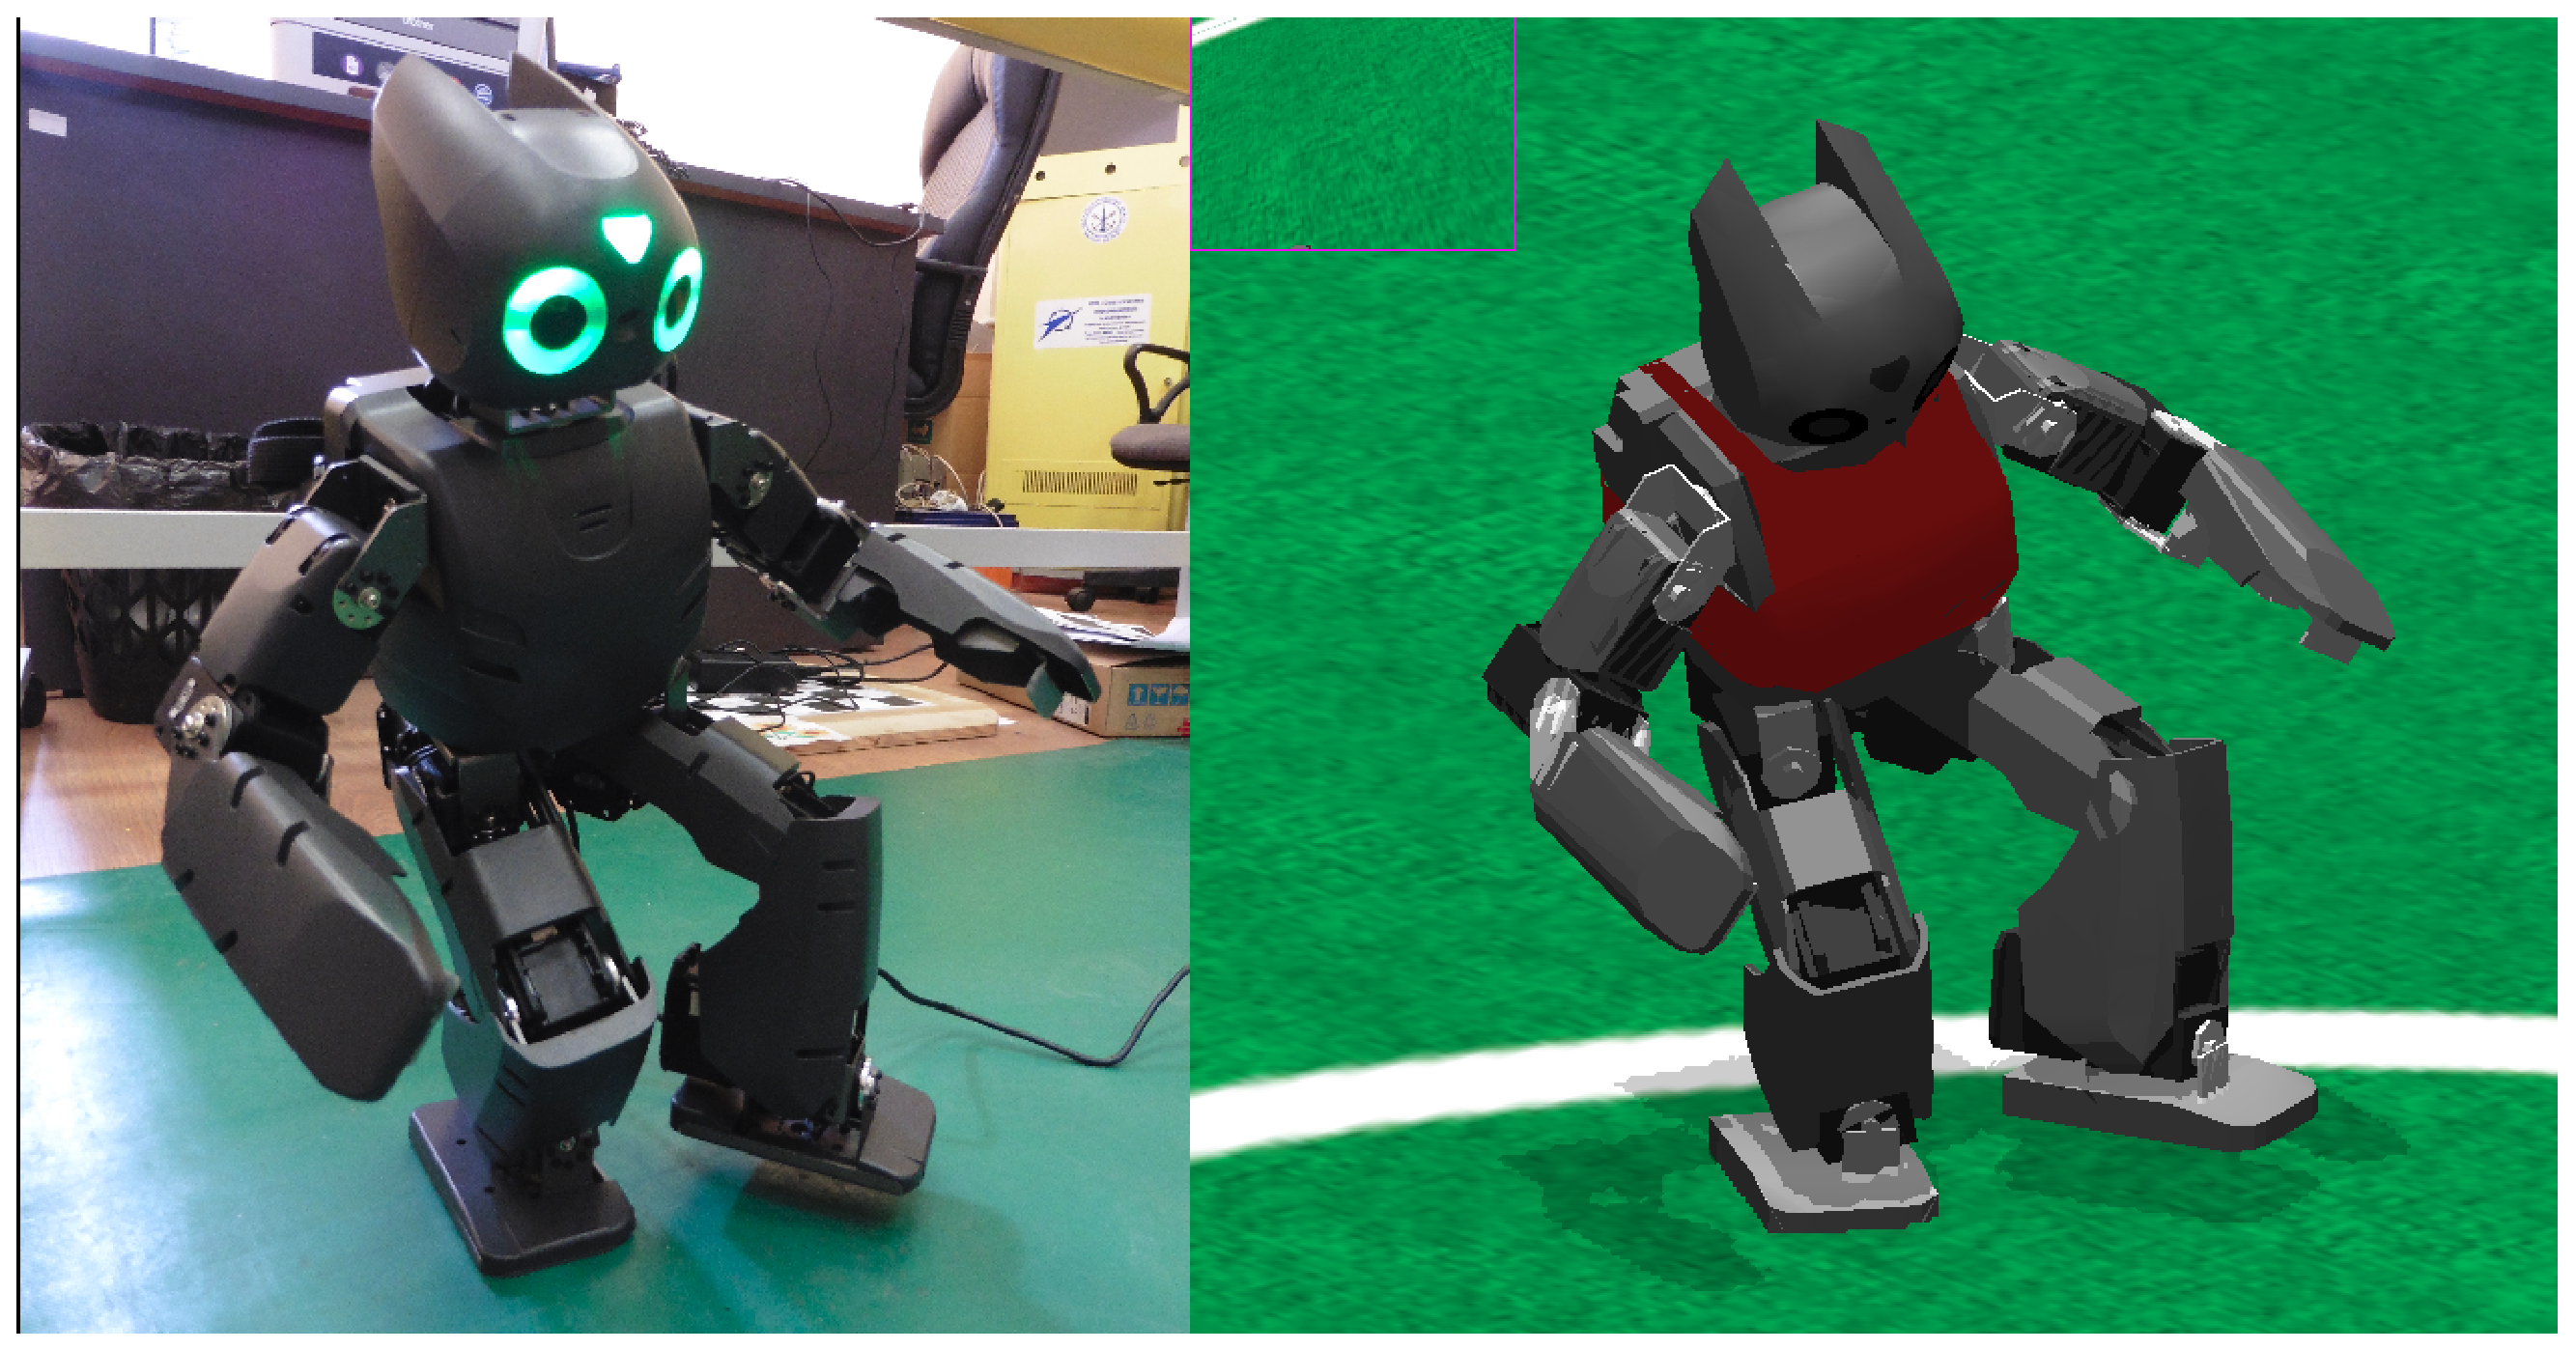
\includegraphics[width=1\linewidth]{2_testing_pose}}
\caption{Тестирование системы управления}
\label{im:2_testing_pose}
\end{figure}

Передача данных на сервоприводы происходит без видимых задержек. Тестирование быстродействия производилось с постоянным изменением положения всех частей тела. Среднее время исполнения метода step (1000 вызовов функции) в симуляционной среде Webots на процессоре  Intel(R) Core(TM) i5-3320M CPU @ 2.60GHz составляет $0.014$мс. На реальном роботе (процессор Intel(R) Atom(TM)  Z530 CPU @ 1.60 GHz) среднее время исполнения метода составляет 1.5мс.

Опытным путем было установлено, что метод step в симуляторе Webots должен вызываться в основном потоке программного контроллера. Вызов метода step в дочерних потоках не изменяет позиции сервоприводов. Причину данной ошибки и способов ее устранения найти не удалось.

Результаты тестирования показали, что реализованный алгоритм управления корректно работает на реальном роботе и в симуляционной среде Webots и устанавливает робота в заданную позицию. Так же реализованный алгоритм имеет высокую производительность и позволяет управлять сервоприводами робота без существенных задержек движения.
